\documentclass{oci}
\usepackage[utf8]{inputenc}
\usepackage{lipsum}
\usepackage{amsmath,amsthm,amsfonts, amssymb}
\usepackage{tikz}

\title{Ocio}

\begin{document}
\begin{problemDescription}

Los organizadores de las olimpiadas de informática se encuentran aburridos mientras su programa está compilando. Para matar el tiempo deciden jugar al juego del OCIo. 

El juego del OCIo consiste en lo siguiente: se comienza con el número $1$, luego alguien lee en voz alta lo que ve: "un uno" y escribe $11$. Luego otro jugador lee en voz alta "dos unos" y escribe $21$, luego el jugador siguiente lee "un dos, un uno" y escribe $1211$. Los OCIosos jugadores continúan. Los primeros números que encontrarán son:

$$1, 11, 21, 1211, 111221, 312211, 13112221, 1113213211, 31131211131221 \dots.$$ 

Para jugar al OCIo, los organizadores escriben los números a medida que aparecen en un computador viejo que tiene una memoria limitada de tamaño $M$. Cada dígito ocupa un espacio de memoria, y cada par de números consecutivos debe estar separado por un espacio, lo cual también ocupa un espacio de memoria.

Los OCIosos programadores se preguntan cuantos números serán capaces de escribir \textbf{completamente} antes de que se les acabe la memoria. Por ejemplo, si $M = 19$, se pueden escribir $5$ números.

\begin{center}
	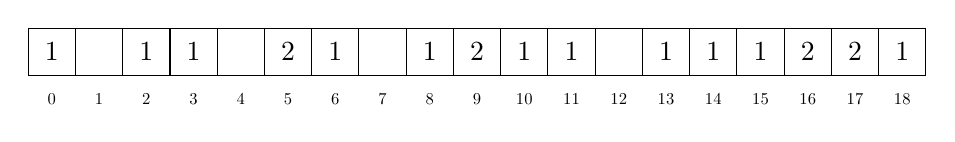
\begin{tikzpicture}[scale = 0.6]
	\foreach \i in {0,...,18}{
		\draw [fill = white] (\i,0) rectangle +(1,1);
		\node at (\i+0.5,-0.5) {\scalebox{0.6}{$\i$}};
	}
	\draw [fill = white] (0,0) rectangle +(1,1);
	\node at (0+0.5,0.5) {$1$};
	\node at (1+0.5,0.5) {$ $};
	\node at (2+0.5,0.5) {$1$};
	\node at (3+0.5,0.5) {$1$};
	\node at (4+0.5,0.5) {$ $};
	\node at (5+0.5,0.5) {$2$};
	\node at (6+0.5,0.5) {$1$};
	\node at (7+0.5,0.5) {$ $};
	\node at (8+0.5,0.5) {$1$};
	\node at (9+0.5,0.5) {$2$};
	\node at (10+0.5,0.5) {$1$};
	\node at (11+0.5,0.5) {$1$};
	\node at (12+0.5,0.5) {$ $};
	\node at (13+0.5,0.5) {$1$};
	\node at (14+0.5,0.5) {$1$};
	\node at (15+0.5,0.5) {$1$};
	\node at (16+0.5,0.5) {$2$};
	\node at (17+0.5,0.5) {$2$};
	\node at (18+0.5,0.5) {$1$};
	\end{tikzpicture}
\end{center}

pero si $M = 18$, tan sólo se podrían escribir $4$ números.

\begin{center}
	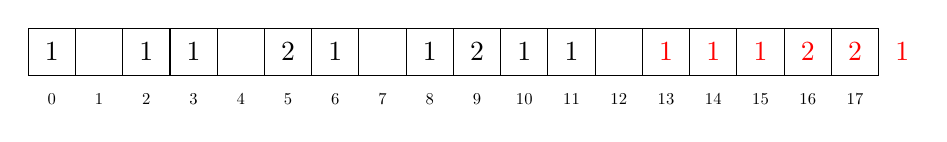
\begin{tikzpicture}[scale = 0.6]
	\foreach \i in {0,...,17}{
		\draw [fill = white] (\i,0) rectangle +(1,1);
		\node at (\i+0.5,-0.5) {\scalebox{0.6}{$\i$}};
	}
	\draw [fill = white] (0,0) rectangle +(1,1);
	\node at (0+0.5,0.5) {$1$};
	\node at (1+0.5,0.5) {$ $};
	\node at (2+0.5,0.5) {$1$};
	\node at (3+0.5,0.5) {$1$};
	\node at (4+0.5,0.5) {$ $};
	\node at (5+0.5,0.5) {$2$};
	\node at (6+0.5,0.5) {$1$};
	\node at (7+0.5,0.5) {$ $};
	\node at (8+0.5,0.5) {$1$};
	\node at (9+0.5,0.5) {$2$};
	\node at (10+0.5,0.5) {$1$};
	\node at (11+0.5,0.5) {$1$};
	\node at (12+0.5,0.5) {$ $};
	\node at (13+0.5,0.5) {${\color{red}1}$};
	\node at (14+0.5,0.5) {${\color{red}1}$};
	\node at (15+0.5,0.5) {${\color{red}1}$};
	\node at (16+0.5,0.5) {${\color{red}2}$};
	\node at (17+0.5,0.5) {${\color{red}2}$};
	\node at (18+0.5,0.5) {${\color{red}1}$};
	\end{tikzpicture}
\end{center}

Ayuda a los Ociosos a encontrar la respuesta que buscan!

\end{problemDescription}

\begin{inputDescription}
El input consiste en un entero $M$ que describe el tamaño de la memoria.
\end{inputDescription}

\begin{outputDescription}
La salida es un entero que describe la cantidad de números de la secuencia que pueden escribirse en la memoria.
\end{outputDescription}

\begin{scoreDescription}
  \score{40} $0 \leq M \leq 100$
  \score{60} $0 \leq M \leq 10^6$
\end{scoreDescription}

\begin{sampleDescription}
\sampleIO{sample-1}
\sampleIO{sample-2}
\end{sampleDescription}

\end{document}
